
\chapter{Reduction}







\section{Introducing Reduction}


Want to formalise our intuition that certain problems are harder than
others. Use notion of \textit{reduction}.

Given two languages: $L_1 \subseteq \Sigma^{*}_1$
and $L_2 \subseteq \Sigma^{*}_2$, a \textit{$\mathcal{C}$-time reduction of $L_1$ to $L_2$}
is defined to be computable function $f : \Sigma^{*}_1 \rightarrow \Sigma^{*}_2$
such that:

\begin{itemize}   
\renewcommand{\labelitemi}{$\Box$}
\item \textbf{Codomain is a subset} The codomain of $f$ is a subset of  $L_2$. 
In other words if instance $x$ is in $L_1$ then there is some instance $f(x)$ in $L_2$. 
And if $f(x)$ is an instance in $L_2$, we will there will be an instance x in $L_1$. 
\item \textbf{Computable in $\mathcal{C}$-time} The function $f$ can be computed 
by our computational model, where $\mathcal{C}$ 
is some language complexity class. 
In other words $f$ is in the \textit{function} complexity class.
\end{itemize} 

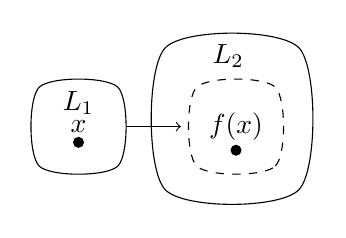
\begin{tikzpicture}
% left
\draw plot [smooth cycle] coordinates {(0,0) (1,0) (1,1) (0,1) };
\node (x) at (0.5,0.5) {$x$};
\fill (x.south) circle [radius=2pt];
\node (x) at (0.5,0.8) {$L_1$};
% right
\node (fx) at (2.5,0.5) {$f(x)$};
\fill (fx.south) circle [radius=2pt];
\draw[dashed] plot [smooth cycle] coordinates {(2,0) (3,0) (3,1) (2,1) };
\draw plot [smooth cycle] coordinates {(1.6,-0.3) (3.3,-0.3) (3.3,1.5) (1.6,1.5) };
\draw[->] (1.1,0.5) -- (1.8,0.5);
\node (x) at (2.4,1.4) {$L_2$};
\end{tikzpicture}


\highlightdef{A \textbf{Reduction in C-time} of 
 $L_1$ to $L_2$ is a computable function in complexity class $C$ that 
 maps every instance of $L_1$ to an instance of $L_2$}

Since we can map every instance of $L_1$ to an instance of $L_2$, 
we can conclude that $L_2$ is either equally hard or harder.


\highlightdef{$L_1$ is \textbf{reducible} 
to $L_2$ in $C$-time, written, $L_1 \leq_{C} L_2$ 
iff there exixts a reduction in $\mathcal{C}$-time of $L_1$ to $L_2$}

\frmrule

\begin{example}
Give a precise definition of what it means for one decision problem to be
polynomial-time reducible to another
\end{example}

\begin{example}
If  $A \subseteq \Sigma^{*}_1$ and $B \subseteq \Sigma^{*}_2$
are two languages over the alphabets $\Sigma_1$ and $\Sigma_2$ respectively,
we write $A \leq_P B$ to denote that $A$ is polynomial-time reducible to $B$.

Is the relation $A \leq_P B$ on languages:
(i) reflexive? (ii) symmetric? (iii) transitive?
Give a proof for your answer in each case.
\end{example}


\begin{example}
Consider the following two decision problems:

\textit{HamCycle}: Given a graph $G = (V,E)$ does it contain a cycle that visits
every vertex exactly once? \\
\textit{HamPath}: Given an undirected simple graph $G = (V,E)$ 
and two distinguished vertices $s, t \in V$, 
is there a simple path in $G$ that starts at $s$, ends at $t$ 
and visits every other vertex exactly once?

Show that \textit{HamCycle} is polynomial-time reducible to \textit{HamPath}
\end{example}

\begin{example}
The following decision problem is known to be solvable in polynomial time:

\textit{EulerCycle}: Given a graph $G = (V, E)$ does it contain a cycle that visits
every edge exactly once?

What can you conclude about the truth of the following statements? Justify
your answers.\\
(a) \textit{EulerCycle} is polynomial-time reducible to \textit{HamCycle}.\\
(b) \textit{EulerCycle} is polynomial-time reducible to \textit{HamPath}.\\
(c) \textit{HamPath} is polynomial-time reducible to \textit{EulerCycle}.
\end{example}


\begin{example}
Prove that for any language $L$, $L$ is polynomial-time reducible to some problem
in \textsc{np} if, and only if, $L$ is in \textsc{np}.
\end{example}


\frmrule

\begin{example}
Recall the following two decision problems:

\textit{HamPath}: Given an undirected simple graph $G = (V,E)$ 
and two distinguished vertices $s, t \in V$, 
is there a simple path in $G$ that starts at $s$, ends at $t$ 
and visits every other vertex exactly once?\\
\textit{LogicSat}: Given a set of clauses, is there an 
assignment for the atoms which makes all the clauses true simultaneously?

We can show that $\text{\textit{HamPath}} \leq_P \text{\textit{LogicSat}}$
\end{example}

\frmrule

\begin{example}
Recall the following two decision problems:

\textit{LogicSat}: Given a set of clauses, is there an 
assignment for the atoms which makes all the clauses true simultaneously? \\
\textit{Logic3Sat}: Given a set of clauses, where every clause has exactly 3 literals, 
is there an assignment for the atoms which makes all the clauses true simultaneously?

We can show that $\text{\textit{LogicSat}} \leq_P \text{\textit{LogicSat3}}$

\frmrule

The reduction relies on two main ideas. 
First we will add new variables $x_i$ so that we will obtain clauses with three literals.
Secondly, we will repeatedly use the lemma $\top = a \vee \neg a$. 
Notice that the following are logically equivalent:



\end{example}


\begin{example}
Recall the following two decision problems:

\textit{LogicSat}: Given a set of clauses, is there an 
assignment for the atoms which makes all the clauses true simultaneously? \\
\textit{VertexCover}$(k)$: Given a graph $G = (V,E)$ and natural number $k$, 
is there a vertex set $X$ with $k$ or less vertices such that for 
every edge $(v_i, v_j)$ in $G$, $v_i \in X$ or $v_j \in X$?


We can show that $\text{\textit{LogicSat}} \leq_P \text{\textit{VertexCover}}$


\end{example}






\section{NP-Completeness}

